\subsubsection{\emph{Process View}}
\label{subsubsec:process-view}

\begin{figure}[htbp]
    \centering
    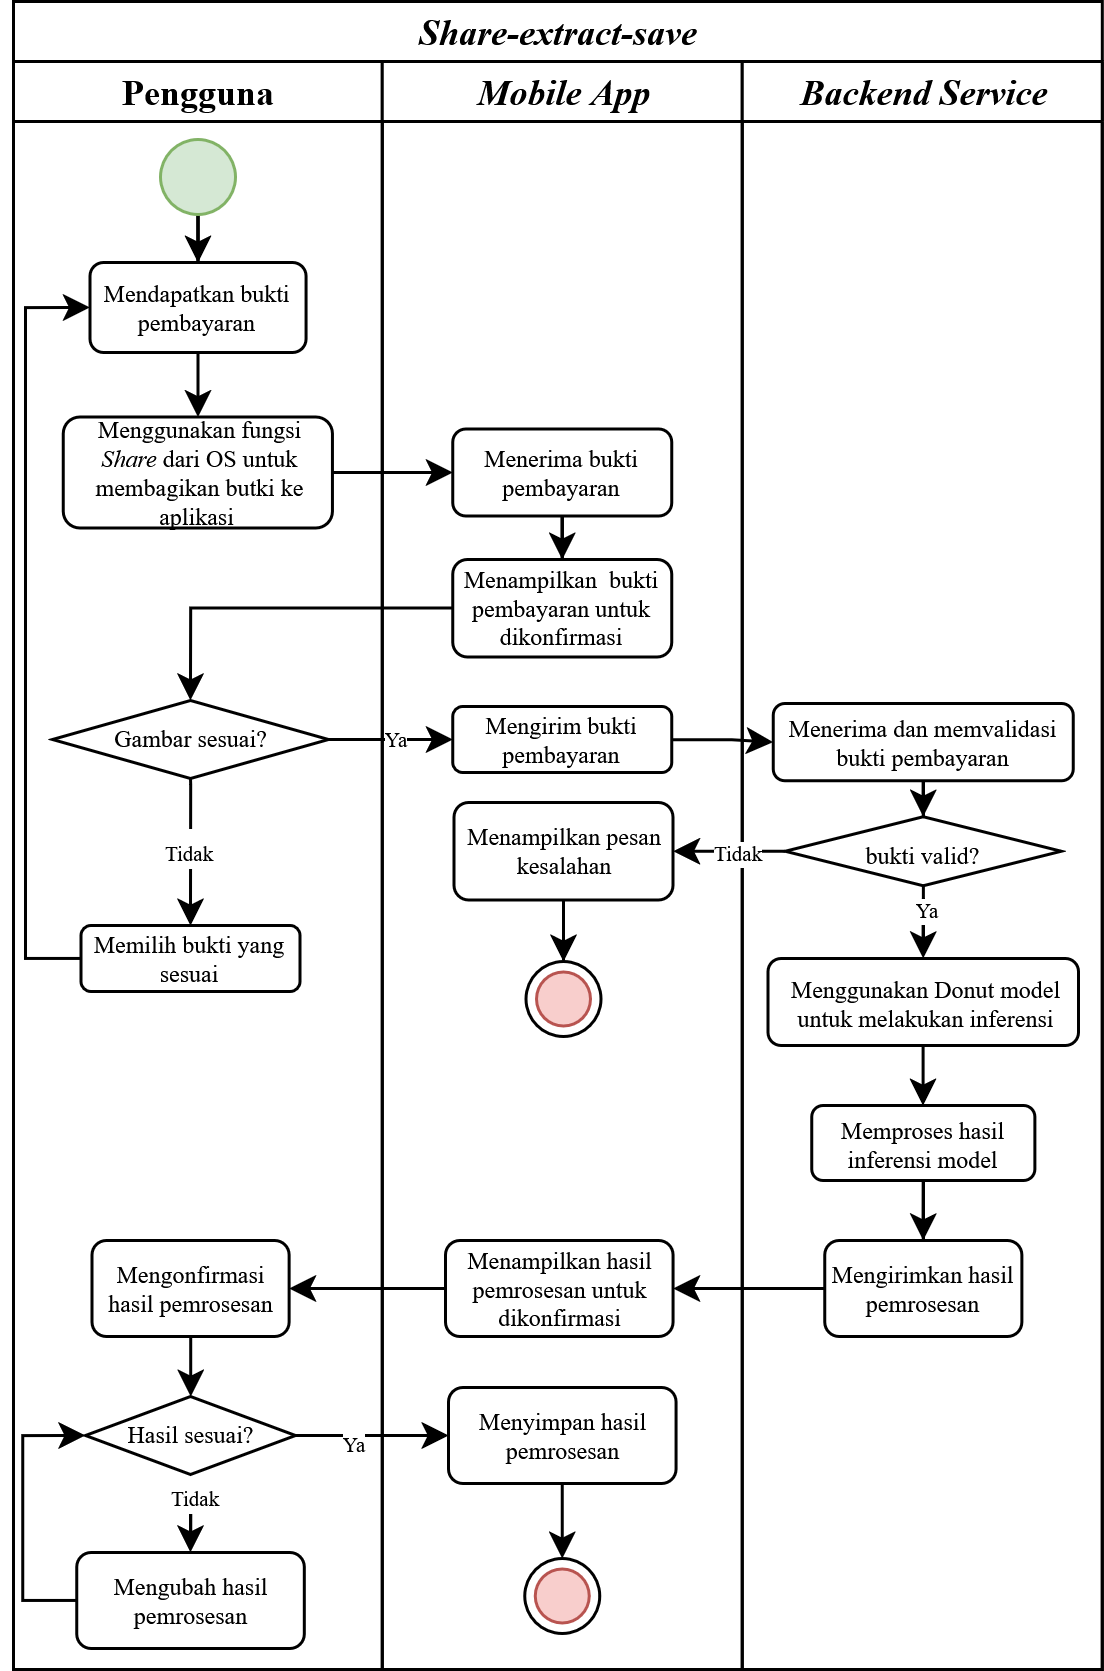
\includegraphics[width=.90625\textwidth]{images/activity-diagram.png}
    \caption{\emph{Activity diagram} untuk proses \emph{share-extract-save}}
    \label{fig:activity-diagram}
\end{figure}

\emph{Process view} menunjukkan alur kerja sistem dalam menangani proses bisnis dari perspektif interaksi antara pengguna dan sistem. \autoref{fig:activity-diagram} menunjukkan \emph{activity diagram} untuk proses \emph{share-extract-save} yang merupakan proses utama dari sistem yang dibangun. Sebelum proses dimulai, pengguna diasumsikan telah melakukan transaksi dan memiliki bukti pembayaran QRIS atau transfer. 

Proses dimulai dengan pengguna memiliki bukti pembayaran dan menggunakan fungsi \emph{share} yang disediakan sistem operasi untuk membagikan artefak tersebut ke aplikasi \emph{mobile}. Aplikasi \emph{mobile} akan menerima artefak tersebut dan menampilkan antarmuka untuk mengonfirmasi artefak yang ingin diproses. Jika artefak sesuai, aplikasi \emph{mobile} akan mengirim bukti pembayaran ke layanan \emph{backend} untuk divalidasi. Jika validasi berhasil, layanan \emph{backend} akan memproses bukti pembayaran dengan menggunakan model \donut{} untuk melakukan inferensi. Hasil inferensi akan diproses untuk menjadi format JSON yang sesuai dan dapat diterima aplikasi \emph{mobile}. Aplikasi \emph{mobile} menampilkan hasil pemrosesan untuk dikonfirmasi. Jika hasil telah sesuai dengan keinginan pengguna, pengguna dapat menyimpan hasil tersebut. Jika hasil pemrosesan masih belum sesuai dengan keinginan pengguna, pengguna masih dapat mengubah hasil ekstraksi dan kemudian menyimpan hasil yang telah diperbaiki.
